\documentclass[10pt]{article}
\usepackage[polish]{babel}
\usepackage[utf8]{inputenc}
\usepackage[T1]{fontenc}
\usepackage{amsmath}
\usepackage{amsfonts}
\usepackage{amssymb}
\usepackage[version=4]{mhchem}
\usepackage{stmaryrd}
\usepackage{graphicx}
\usepackage[export]{adjustbox}
\graphicspath{ {./images/} }

\title{KLASY PO SZKOLE PODSTAWOWEJ }

\author{}
\date{}


\begin{document}
\maketitle
Zestaw 21

\begin{enumerate}
  \item Zegar pokazuje godzinę 6:00. Po jakim czasie długa wskazówka dogoni krótką?
  \item 5 pająków łapie 5 much w ciągu pięciu godzin. Ile much łapie 100 pająków w ciągu 100 godzin?
  \item W trójkącie ostrokątnym \(A B C\) poprowadzono wysokość CD. Punkt E należy do boku AC, a odcinki BE i CD przecinają się w punkcie H, przy czym wiadomo, że CD = DB i HD = DA. Wykaż, że odcinek BE jest wysokością trójkąta ABC.\\
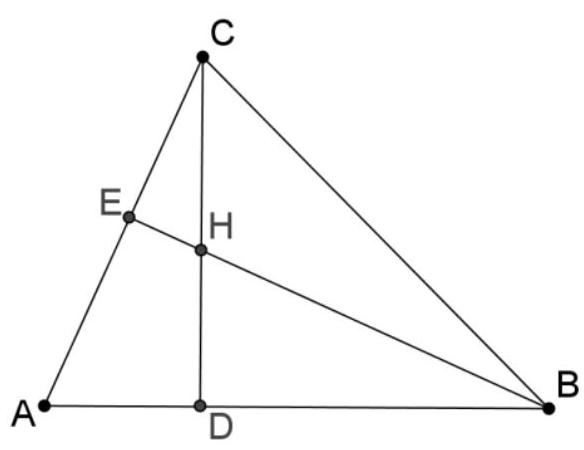
\includegraphics[max width=\textwidth, center]{2024_11_21_b91e86a5070ac23144a8g-1(1)}
\end{enumerate}

\section*{KLASY PO GIMNAZJUM}
\begin{enumerate}
  \item Wyznacz kąty trójkąta \(A B C\), którego wysokość \(C D\) i dwusieczna BE przecinają się w takim punkcie M, że \(\mathrm{CM}=2 \mathrm{DM}\) i BM = ME.
  \item Rozstrzygnij, czy istnieje taka liczba naturalna \(n\), dla której liczby \(\sqrt[6]{6 n} ; \sqrt[8]{8 n}\) są naturalne.\\
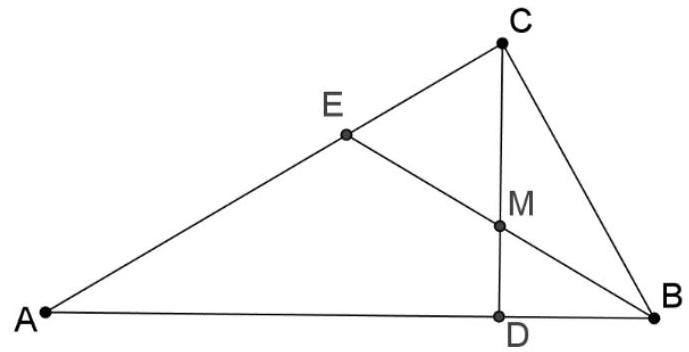
\includegraphics[max width=\textwidth, center]{2024_11_21_b91e86a5070ac23144a8g-1}
  \item Udowodnij, że dla dowolnych liczb dodatnich \(a, b, c\), zachodzi nierówność:
\end{enumerate}

\[
\left(a^{3}+b^{3}+c^{3}\right)\left(\frac{1}{a}+\frac{1}{b}+\frac{1}{c}\right) \geq(a+b+c)^{2}
\]


\end{document}